\documentclass[border={8pt 6pt 8pt 6pt}]{standalone}
% Gemeinsamer Preamble fuer die Standalone-Grafiken der Schlusspraesentation.
% Pakete gespiegelt aus src/thesis/hslu_thesis.tex (Z. 56-60), damit die
% extrahierten TikZ-/pgfplots-Grafiken identisch zur Arbeit rendern.
\usepackage[T1]{fontenc}
\usepackage[utf8]{inputenc}
\usepackage{tikz}
\usepackage{pgfplots}
\pgfplotsset{compat=1.18}
\usepgfplotslibrary{groupplots}
\usetikzlibrary{patterns}

\begin{document}
% Extrahiert 1:1 aus chapters/06_validation_und_evaluation.tex (fig:eval_openworld_pr).
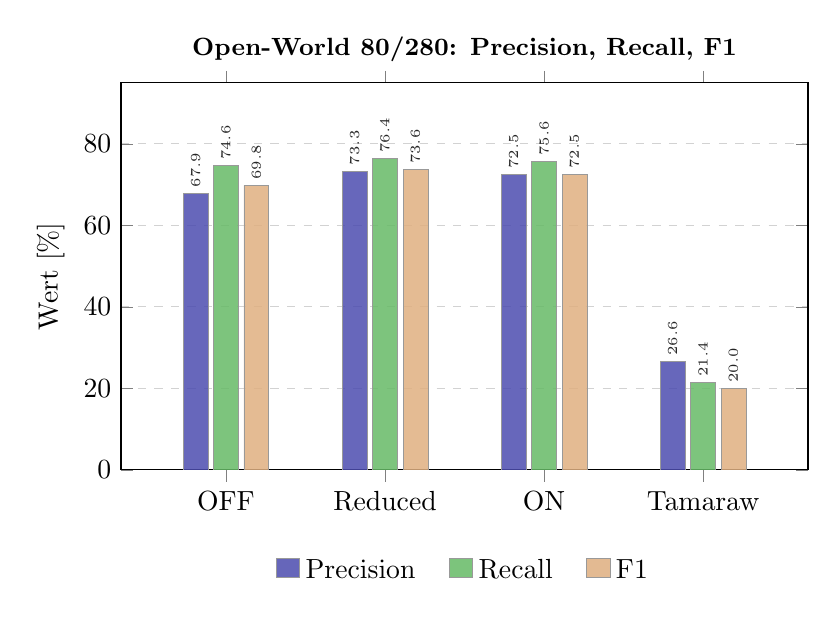
\begin{tikzpicture}
    \begin{axis}[
        ybar,
        title={Open-World 80/280: Precision, Recall, F1},
        title style={font=\small\bfseries, yshift=-2pt},
        width=0.85\textwidth,
        height=6.5cm,
        bar width=9pt,
        ymin=0, ymax=95,
        ylabel={Wert [\%]},
        symbolic x coords={OFF, Reduced, ON, Tamaraw},
        xtick=data,
        enlarge x limits=0.22,
        ymajorgrids=true,
        grid style={dashed, gray!35},
        legend style={at={(0.5,-0.20)}, anchor=north, legend columns=3, draw=none, /tikz/every even column/.append style={column sep=10pt}},
        legend image code/.code={\draw[#1, draw=black!40, line width=0.3pt] (0cm,-0.08cm) rectangle (0.3cm,0.16cm);},
        nodes near coords,
        nodes near coords style={font=\tiny, rotate=90, anchor=west, inner sep=2pt, /pgf/number format/.cd, fixed, fixed zerofill, precision=1},
        every axis plot/.append style={fill opacity=0.85, draw=black!40, line width=0.3pt},
        tick style={black!50},
    ]
        \addplot[fill=blue!55!black!70]   coordinates {(OFF,67.9) (Reduced,73.3) (ON,72.5) (Tamaraw,26.6)};
        \addplot[fill=green!55!black!60]  coordinates {(OFF,74.6) (Reduced,76.4) (ON,75.6) (Tamaraw,21.4)};
        \addplot[fill=orange!75!black!50] coordinates {(OFF,69.8) (Reduced,73.6) (ON,72.5) (Tamaraw,20.0)};
        \legend{Precision, Recall, F1}
    \end{axis}
\end{tikzpicture}
\end{document}
